\icode{E-MI-SI-L3-261108-002}
如图，穿在一根固定杆上的两个小球\(A\)，\(B\)连接在一条跨过定滑轮的轻绳两端，杆与水平面的夹角\(\theta =\)\,\qty{30}{\degree}。当两球静止时，绳\(OA\)与杆的夹角也为\(\theta\)，绳\(OB\)沿竖直方向，不计一切摩擦，则球\(A\)，\(B\)的质量之比为\paren[]

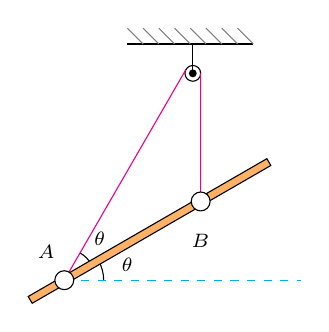
\begin{tikzpicture}[font=\scriptsize]
	\draw (60:.4) arc(60:30:.4);
	\draw (.5,0) arc(0:30:.5);
	\begin{scope}[rotate=30]
		\coordinate (O) at(0,0);
		\coordinate (A) at(2,0);
		\draw[fill=orange!60] (-.5,-.05) rectangle(3,.05);
	\end{scope}
	\coordinate (C) at({sqrt(3)-.1},{3-.1/tan(15)});
	\coordinate (D) at({sqrt(3)},{3-.1/tan(15)});
	\coordinate (E) at({0.95*sqrt(3)-.1},{3.05-.1/tan(15)});
	\draw (C) circle(.1);
	\fill (C) circle(.05);
	\draw[dashed,cyan] (0,0)--(3,0);
	\draw[magenta] (O)--(E) (D)--(A);
    \draw (.8,3)--(2.4,3) (C)--(C|-0,3);
	\draw[fill=white] (O) circle(.12) (A) circle(.12);
	\foreach \x in {.8,1,...,2.2}
		\draw[gray] (\x,3.2)--++(.2,-.2);
	\node at(.8,.2){\(\theta\)};
	\node at(.45,.52){\(\theta\)};
	\node at(0,.15)[above left]{\(A\)};
	\node at(1.73,.5){\(B\)};
\end{tikzpicture}	
\begin{choices}
	\item\(\sqrt{3}:1\)
	\item\(1:\sqrt{3}\)
	\item\(2:\sqrt{3}\)
	\item\(\sqrt{3}:2\)
\end{choices}		
\begin{answer}
	A\qquad 提示：
\end{answer}